\documentclass{beamer}
\usetheme{Madrid}
\usecolortheme{whale}
\usepackage{amsmath,amssymb}
\usepackage{graphicx}
\usepackage{tikz}
\usetikzlibrary{positioning,arrows.meta,shapes}
\usepackage{algorithm}
\usepackage{algorithmic}
\usepackage{booktabs}

\title{Extending the Toy Model: From Single Measurements to Hierarchical Distributions}
\subtitle{A Roadmap for Bayesian Hierarchical Modeling of Protein Assemblies}
\author{Researcher}
\date{\today}

\begin{document}

\frame{\titlepage}

% Slide 1: Current Problem Analysis
\begin{frame}{Current Limitations and Required Changes}
\framesubtitle{Why the current approach hasn't worked}

\textbf{What I've been doing (and why it failed):}
\begin{itemize}
    \item Using single distance measurements (AA=15Å, AB=20Å, BC=18Å)
    \item Reusing same 3 data points across stages 1-3
    \item Trying to infer 3 uncertainty parameters from 3 measurements
\end{itemize}

\vspace{0.5cm}
\textbf{Why this doesn't work:}
\begin{itemize}
    \item \textcolor{red}{Underdetermined system}: $\sigma$ parameters have no variance to explain
    \item \textcolor{red}{No information gain}: Each stage sees identical data
    \item \textcolor{red}{No hierarchical learning}: Cannot demonstrate "borrowing of strength"
\end{itemize}

\vspace{0.5cm}
\textbf{The fix:} Generate distributional data at each hierarchical level with realistic noise models
\end{frame}

% Slide 2: New Data Generation Strategy
\begin{frame}{Revised Data Generation Strategy}
\framesubtitle{Creating meaningful hierarchical data}

\begin{columns}
\column{0.5\textwidth}
\textbf{Stage 1: Intra-subunit}
\begin{itemize}
    \item \textcolor{blue}{20 measurements} per distance type
    \item AA: $15.0 \pm 0.5$ Å
    \item AB: $20.0 \pm 0.8$ Å  
    \item BC: $18.0 \pm 0.6$ Å
\end{itemize}

\textbf{Stage 2: Inter-subunit (within tetramer)}
\begin{itemize}
    \item \textcolor{blue}{15 measurements} per pair
    \item A-A': $25.0 \pm 1.5$ Å
    \item B-B': $30.0 \pm 2.0$ Å
\end{itemize}

\column{0.5\textwidth}
\textbf{Stage 3: Inter-tetramer}
\begin{itemize}
    \item \textcolor{blue}{10 measurements}
    \item Tetramer COM: $45.0 \pm 3.0$ Å
    \item Higher noise (longer range)
\end{itemize}

\textbf{Stage 4: Global (Cryo-EM)}
\begin{itemize}
    \item 3D density map
    \item 5Å resolution
    \item Different data type entirely
\end{itemize}
\end{columns}

\vspace{0.3cm}
\textbf{Key principle:} Measurement precision decreases with distance scale
\end{frame}

% Slide 3: Hierarchical Model Structure
\begin{frame}{Hierarchical Model Architecture}
\framesubtitle{How parameters are connected across stages}

\begin{center}
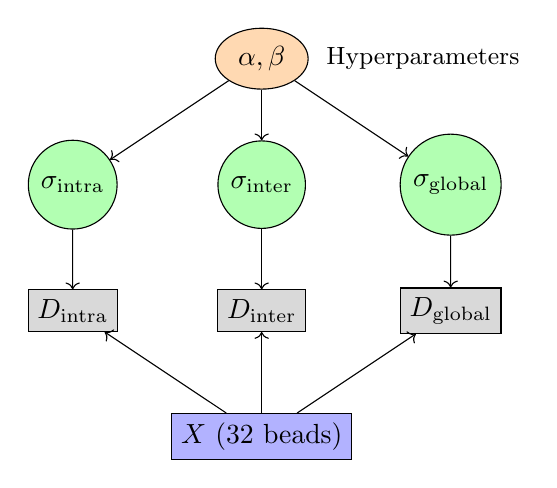
\begin{tikzpicture}[scale=0.8]
    % Hyperparameters
    \node[ellipse,draw,fill=orange!30] (alpha) at (0,4) {$\alpha, \beta$};
    \node[right=0.1cm of alpha] {\small Hyperparameters};
    
    % Stage-specific parameters
    \node[circle,draw,fill=green!30] (s1) at (-3,2) {$\sigma_{\text{intra}}$};
    \node[circle,draw,fill=green!30] (s2) at (0,2) {$\sigma_{\text{inter}}$};
    \node[circle,draw,fill=green!30] (s3) at (3,2) {$\sigma_{\text{global}}$};
    
    % Data
    \node[rectangle,draw,fill=gray!30] (d1) at (-3,0) {$D_{\text{intra}}$};
    \node[rectangle,draw,fill=gray!30] (d2) at (0,0) {$D_{\text{inter}}$};
    \node[rectangle,draw,fill=gray!30] (d3) at (3,0) {$D_{\text{global}}$};
    
    % Structure
    \node[rectangle,draw,fill=blue!30] (X) at (0,-2) {$X$ (32 beads)};
    
    % Arrows
    \draw[->] (alpha) -- (s1);
    \draw[->] (alpha) -- (s2);
    \draw[->] (alpha) -- (s3);
    \draw[->] (s1) -- (d1);
    \draw[->] (s2) -- (d2);
    \draw[->] (s3) -- (d3);
    \draw[->] (X) -- (d1);
    \draw[->] (X) -- (d2);
    \draw[->] (X) -- (d3);
\end{tikzpicture}
\end{center}

\textbf{What this achieves:}
\begin{itemize}
    \item All $\sigma$ parameters share hyperpriors: $\sigma_k^2 \sim \text{InverseGamma}(\alpha, \beta)$
    \item Information about precision at one scale informs others
    \item Can learn that $\sigma_{\text{intra}} < \sigma_{\text{inter}} < \sigma_{\text{global}}$
\end{itemize}
\end{frame}

% Slide 4: Implementation Plan
\begin{frame}{Implementation Action Plan}
\framesubtitle{Concrete steps I will take}

\begin{enumerate}
    \item \textbf{Week 1-2: Data Generation}
    \begin{itemize}
        \item Generate synthetic measurements with realistic noise
        \item Create 100 datasets for validation
        \item Implement data likelihood functions for each type
    \end{itemize}
    
    \item \textbf{Week 3-4: Scoring Functions}
    \begin{itemize}
        \item Intra-subunit: Harmonic restraints
        \item Inter-subunit: Flat-bottom restraints  
        \item Inter-tetramer: Ambiguous distance restraints
    \end{itemize}
    
    \item \textbf{Week 5-6: Sampling Implementation}
    \begin{itemize}
        \item Implement GMM fitting with EM algorithm
        \item Add adaptive MCMC proposals
        \item Implement convergence diagnostics
    \end{itemize}
    
    \item \textbf{Week 7-8: Validation}
    \begin{itemize}
        \item Compare sequential vs full BHM
        \item Quantify information loss through KL divergence
        \item Test on perturbed ground truth structures
    \end{itemize}
\end{enumerate}
\end{frame}

% Slide 5: Scoring Function Details
\begin{frame}{Stage-Specific Scoring Functions}
\framesubtitle{Mathematical formulations I will implement}

\textbf{Stage 1 - Intra-subunit (Harmonic):}
$$p(d_{ij}^{\text{obs}} | d_{ij}^{\text{calc}}, \sigma_{\text{intra}}) = \prod_{k=1}^{20} \mathcal{N}(d_{ij,k}^{\text{obs}} | d_{ij}^{\text{calc}}, \sigma_{\text{intra}}^2)$$

\textbf{Stage 2 - Inter-subunit (Flat-bottom):}
$$p(d_{ij}^{\text{obs}} | d_{ij}^{\text{calc}}, \sigma_{\text{inter}}) = \begin{cases}
1 & \text{if } |d_{ij}^{\text{calc}} - d_{ij}^{\text{obs}}| < \delta \\
\exp(-\frac{(|d_{ij}^{\text{calc}} - d_{ij}^{\text{obs}}| - \delta)^2}{2\sigma_{\text{inter}}^2}) & \text{otherwise}
\end{cases}$$

\textbf{Stage 3 - Inter-tetramer (Ambiguous):}
$$p(d^{\text{obs}} | X, \sigma_{\text{global}}) = \sum_{(i,j) \in \text{pairs}} w_{ij} \cdot \mathcal{N}(d^{\text{obs}} | d_{ij}^{\text{calc}}, \sigma_{\text{global}}^2)$$

where $w_{ij}$ are assignment probabilities
\end{frame}

% Slide 6: Expected Outcomes
\begin{frame}{Expected Outcomes and Success Metrics}
\framesubtitle{How I will know the approach works}

\begin{columns}
\column{0.5\textwidth}
\textbf{Convergence Metrics:}
\begin{itemize}
    \item $\hat{R} < 1.01$ for all parameters
    \item ESS $> 200$ per parameter
    \item Stable $\sigma$ posteriors
\end{itemize}

\textbf{Structural Accuracy:}
\begin{itemize}
    \item RMSD $< 2$Å to ground truth
    \item Correct 8-fold symmetry
    \item Proper subunit orientations
\end{itemize}

\column{0.5\textwidth}
\textbf{Information Flow:}
\begin{itemize}
    \item KL divergence decreases per stage
    \item Uncertainty parameters show: $$\sigma_{\text{intra}} < \sigma_{\text{inter}} < \sigma_{\text{global}}$$
    \item GMM captures $>90\%$ of variance
\end{itemize}

\textbf{Computational:}
\begin{itemize}
    \item $<1$ hour per stage
    \item Memory $<$ 8GB
    \item Parallelizable to 8 cores
\end{itemize}
\end{columns}

\vspace{0.5cm}
\textbf{Key validation:} Sequential approximation should achieve 80\% of full BHM accuracy at 20\% computational cost
\end{frame}

% Slide 7: Debugging Strategy
\begin{frame}{Debugging Strategy}
\framesubtitle{How I will diagnose and fix issues}

\begin{enumerate}
    \item \textbf{Start with perfect data}
    \begin{itemize}
        \item No noise initially - verify assembly works
        \item Gradually increase noise levels
        \item Identify breaking points
    \end{itemize}
    
    \item \textbf{Ablation studies}
    \begin{itemize}
        \item Test each stage independently first
        \item Verify GMM approximation quality at each stage
        \item Check information propagation with fixed structures
    \end{itemize}
    
    \item \textbf{Diagnostic plots I will generate:}
    \begin{itemize}
        \item Trace plots for $\sigma$ parameters
        \item Posterior vs prior distributions at each stage
        \item Residual distributions per data type
        \item Energy landscape visualization
    \end{itemize}
    
    \item \textbf{Common failure modes to check:}
    \begin{itemize}
        \item Label switching in GMM
        \item Mode collapse in sampling
        \item Numerical instabilities in likelihood
    \end{itemize}
\end{enumerate}
\end{frame}

% Slide 8: Extension to Real Complexes - Overview
\begin{frame}{Extension to Real Protein Complexes}
\framesubtitle{Bridging from toy model to biological systems}

\begin{center}
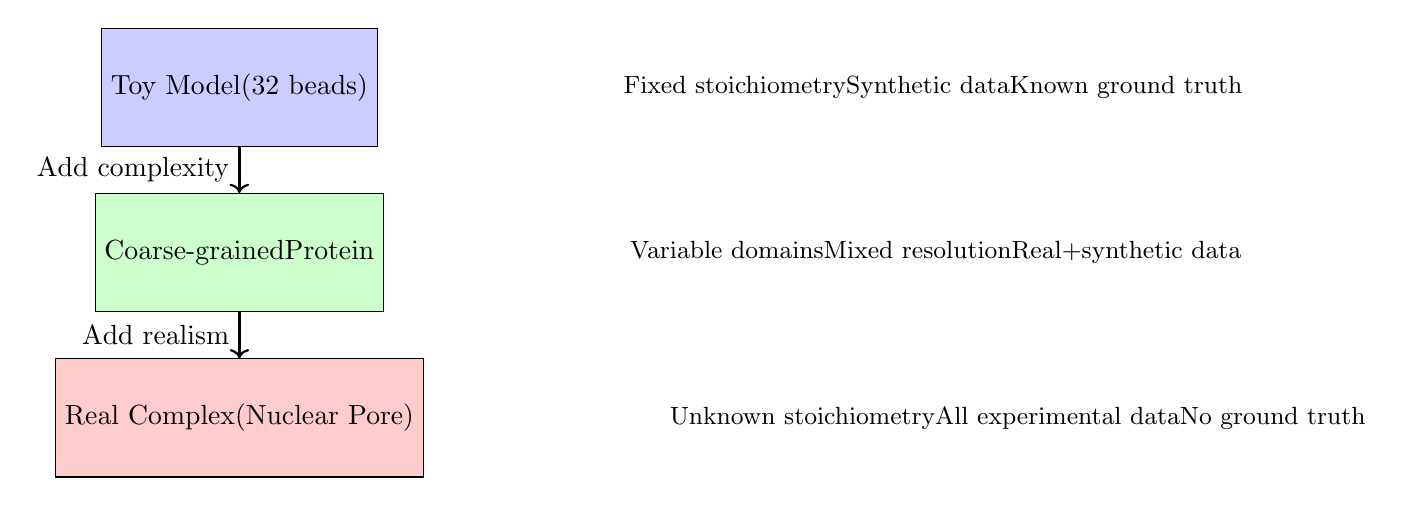
\begin{tikzpicture}[scale=0.7]
    % Toy model
    \node[rectangle,draw,fill=blue!20,minimum width=3cm,minimum height=1.5cm] (toy) at (0,3) {Toy Model\\(32 beads)};
    
    % Intermediate
    \node[rectangle,draw,fill=green!20,minimum width=3cm,minimum height=1.5cm] (inter) at (0,0) {Coarse-grained\\Protein};
    
    % Real complex
    \node[rectangle,draw,fill=red!20,minimum width=3cm,minimum height=1.5cm] (real) at (0,-3) {Real Complex\\(Nuclear Pore)};
    
    % Annotations
    \node[right=3cm of toy] {\small Fixed stoichiometry\\Synthetic data\\Known ground truth};
    \node[right=3cm of inter] {\small Variable domains\\Mixed resolution\\Real+synthetic data};
    \node[right=3cm of real] {\small Unknown stoichiometry\\All experimental data\\No ground truth};
    
    % Arrows
    \draw[->,thick] (toy) -- (inter) node[midway,left] {Add complexity};
    \draw[->,thick] (inter) -- (real) node[midway,left] {Add realism};
\end{tikzpicture}
\end{center}

\textbf{Key capabilities to develop:}
\begin{itemize}
    \item Handle missing data and outliers
    \item Integrate heterogeneous data types
    \item Model compositional heterogeneity
\end{itemize}
\end{frame}

% Slide 9: Real Data Integration
\begin{frame}{Integrating Experimental Data Types}
\framesubtitle{How each data type maps to the hierarchical model}

\begin{table}
\centering
\small
\begin{tabular}{lll}
\toprule
\textbf{Data Type} & \textbf{Information Level} & \textbf{Uncertainty Scale} \\
\midrule
XL-MS & Local (20-30Å) & $\sigma \sim 2-3$Å \\
FRET & Pairwise (30-80Å) & $\sigma \sim 5-10$Å \\
SAXS & Global shape & $\sigma \sim 10\%$ of $R_g$ \\
Cryo-EM & Full structure & Resolution-dependent \\
NMR NOE & Local ($<6$Å) & $\sigma \sim 0.5-1$Å \\
Genetic interactions & Functional proximity & $\sigma$ learned \\
\bottomrule
\end{tabular}
\end{table}

\textbf{Implementation strategy:}
\begin{enumerate}
    \item Start with most reliable data (NMR if available)
    \item Add complementary data types sequentially
    \item Use hyperpriors to learn relative data quality:
    $$\sigma_{\text{XL-MS}}^2, \sigma_{\text{FRET}}^2, \sigma_{\text{SAXS}}^2 \sim \text{InverseGamma}(\alpha, \beta)$$
\end{enumerate}

\textbf{This approach will handle:} Missing data, conflicting measurements, and varying data quality
\end{frame}

% Slide 10: Compositional Heterogeneity
\begin{frame}{Handling Compositional Heterogeneity}
\framesubtitle{When stoichiometry is unknown}

\textbf{The challenge:} Real complexes have variable copy numbers

\textbf{My solution:} Trans-dimensional MCMC with hierarchical priors
\begin{align}
N_{\text{Nup84}} &\sim \text{Poisson}(\lambda_{\text{scaffold}}) \\
N_{\text{Nup85}} &\sim \text{Poisson}(\lambda_{\text{scaffold}}) \\
N_{\text{FG-Nups}} &\sim \text{Poisson}(\lambda_{\text{flexible}})
\end{align}

where $\lambda_{\text{scaffold}} > \lambda_{\text{flexible}}$ (structural vs regulatory)

\textbf{Implementation plan:}
\begin{itemize}
    \item Use reversible jump MCMC for dimension changes
    \item Employ parallel tempering for better mixing
    \item Validate on complexes with known variable stoichiometry (e.g., clathrin coats)
\end{itemize}

\textbf{Success metric:} Correctly infer known stoichiometry ranges from data
\end{frame}

% Slide 11: Computational Scaling
\begin{frame}{Computational Scaling Strategy}
\framesubtitle{Making it practical for large complexes}

\begin{columns}
\column{0.5\textwidth}
\textbf{Problem sizes:}
\begin{itemize}
    \item Toy model: 32 beads
    \item Small protein: 500 beads
    \item NPC spoke: 5,000 beads
    \item Full NPC: 50,000 beads
\end{itemize}

\textbf{Scaling approach:}
\begin{itemize}
    \item Hierarchical representation
    \item GPU acceleration for distances
    \item Sparse restraint matrices
    \item Checkpointing for recovery
\end{itemize}

\column{0.5\textwidth}
\begin{center}
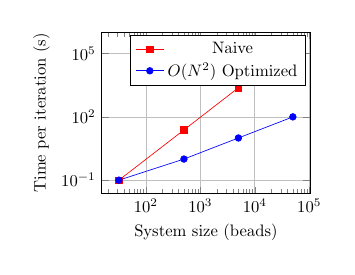
\begin{tikzpicture}[scale=0.6]
    \begin{axis}[
        xlabel={System size (beads)},
        ylabel={Time per iteration (s)},
        xmode=log,
        ymode=log,
        grid=major,
        width=6cm,
        height=5cm
    ]
    % Naive
    \addplot[color=red,mark=square*] coordinates {
        (32,0.1) (500,24) (5000,2400) (50000,240000)
    };
    % Optimized
    \addplot[color=blue,mark=*] coordinates {
        (32,0.1) (500,1) (5000,10) (50000,100)
    };
    \legend{Naive,$O(N^2)$ Optimized}
    \end{axis}
\end{tikzpicture}
\end{center}
\end{columns}

\textbf{Key optimizations I will implement:}
\begin{itemize}
    \item Distance cutoffs for non-interacting pairs
    \item Locality-sensitive hashing for neighbor lists
    \item Gradient caching for repeated calculations
\end{itemize}
\end{frame}

% Slide 12: Software Architecture
\begin{frame}{Software Architecture Plan}
\framesubtitle{Building a reusable framework}

\begin{center}
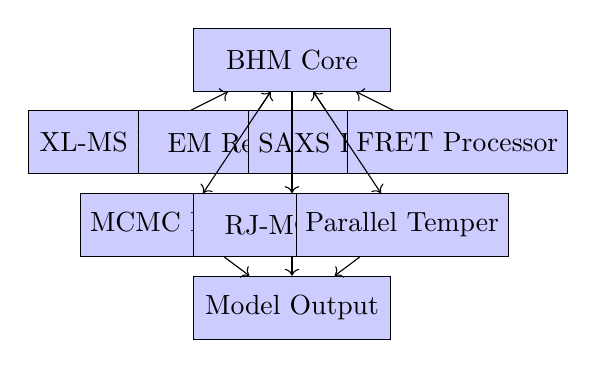
\begin{tikzpicture}[scale=0.7,
    box/.style={rectangle,draw,fill=blue!20,minimum width=2.5cm,minimum height=0.8cm}]
    
    % Core layer
    \node[box] (core) at (0,3) {BHM Core};
    
    % Data handlers
    \node[box] (xlms) at (-3,1.5) {XL-MS Parser};
    \node[box] (em) at (-1,1.5) {EM Reader};
    \node[box] (saxs) at (1,1.5) {SAXS Handler};
    \node[box] (fret) at (3,1.5) {FRET Processor};
    
    % Samplers
    \node[box] (mcmc) at (-2,0) {MCMC Engine};
    \node[box] (rjmcmc) at (0,0) {RJ-MCMC};
    \node[box] (pt) at (2,0) {Parallel Temper};
    
    % Output
    \node[box] (out) at (0,-1.5) {Model Output};
    
    % Connections
    \draw[->] (xlms) -- (core);
    \draw[->] (em) -- (core);
    \draw[->] (saxs) -- (core);
    \draw[->] (fret) -- (core);
    \draw[->] (core) -- (mcmc);
    \draw[->] (core) -- (rjmcmc);
    \draw[->] (core) -- (pt);
    \draw[->] (mcmc) -- (out);
    \draw[->] (rjmcmc) -- (out);
    \draw[->] (pt) -- (out);
\end{tikzpicture}
\end{center}

\textbf{Design principles:}
\begin{itemize}
    \item Modular data handlers for each experimental type
    \item Pluggable sampling strategies
    \item Standardized model representation (mmCIF compatible)
    \item Comprehensive logging and checkpointing
\end{itemize}
\end{frame}

% Slide 13: Validation on Known Structures
\begin{frame}{Validation Strategy for Real Complexes}
\framesubtitle{Testing on structures with known answers}

\textbf{Test cases I will use:}
\begin{enumerate}
    \item \textbf{Proteasome} (Known structure, stable)
    \begin{itemize}
        \item Generate synthetic data from PDB structure
        \item Add realistic noise
        \item Verify recovery of correct architecture
    \end{itemize}
    
    \item \textbf{Ribosome} (Multiple conformations)
    \begin{itemize}
        \item Test ensemble representation
        \item Validate against known states
    \end{itemize}
    
    \item \textbf{Nuclear Pore (Spoke)} (Partial symmetry)
    \begin{itemize}
        \item Test symmetry detection
        \item Handle missing densities
    \end{itemize}
\end{enumerate}

\textbf{Success metrics:}
\begin{itemize}
    \item Correct topology: $>95\%$ contacts recovered
    \item Accurate geometry: RMSD $<$ resolution of input data
    \item Proper uncertainty: Credible intervals contain true structure
\end{itemize}
\end{frame}

% Slide 14: Timeline and Milestones
\begin{frame}{Complete Timeline and Milestones}
\framesubtitle{From toy model to publication}

\textbf{Phase 1: Fix toy model (Months 1-2)}
\begin{itemize}
    \item Week 1-2: Implement distributional data
    \item Week 3-4: Validate BHM approximation
    \item Week 5-6: Achieve reliable assembly
    \item Week 7-8: Document and package
\end{itemize}

\textbf{Phase 2: Extend to proteins (Months 3-4)}
\begin{itemize}
    \item Coarse-grain real proteins
    \item Integrate XL-MS and SAXS data
    \item Validate on known structures
\end{itemize}

\textbf{Phase 3: Real application (Months 5-6)}
\begin{itemize}
    \item Apply to novel complex
    \item Compare with AlphaFold predictions
    \item Prepare publication
\end{itemize}

\textbf{Deliverables:}
\begin{itemize}
    \item Open-source software package
    \item Benchmark dataset
    \item Methods paper + biological application
\end{itemize}
\end{frame}

% Slide 15: Conclusions
\begin{frame}{Summary and Next Steps}
\framesubtitle{The path forward is clear}

\textbf{What I've learned:}
\begin{itemize}
    \item Single measurements cannot constrain uncertainty parameters
    \item Hierarchical data structure is essential for BHM
    \item Sequential approximation requires careful validation
\end{itemize}

\textbf{What I will do immediately:}
\begin{enumerate}
    \item Generate proper distributional data for toy model
    \item Implement stage-specific scoring functions
    \item Validate information flow between stages
    \item Quantify approximation quality
\end{enumerate}

\textbf{Long-term vision:}
\begin{itemize}
    \item Create a general framework for integrative modeling
    \item Enable structure determination of heterogeneous complexes
    \item Bridge computational and experimental structural biology
\end{itemize}

\vspace{0.5cm}
\centering
\textbf{\large The key insight: Match the data hierarchy to the model hierarchy}
\end{frame}

\end{document}